%%%%%%%%%%%%%%%%%%%%%%%%%%%%%%%%%%%%%%%%%%
% Engineering problems / LaTeX Template
%		Semester 5
%		Institut d'Optique Graduate School
%%%%%%%%%%%%%%%%%%%%%%%%%%%%%%%%%%%%%%%%%%
%	5N-OptoElec-Sujet	
%%%%%%%%%%%%%%%%%%%%%%%%%%%%%%%%%%%%%%%%%%
%
% Created by:
%	Julien VILLEMEJANE - 05/may/2025
%	
%
%%%%%%%%%%%%%%%%%%%%%%%%%%%%%%%%%%%%%%%%%%
% Professional Newsletter Template
% LaTeX Template
% Version 1.0 (09/03/14)
%
% Created by:
% Bob Kerstetter (https://www.tug.org/texshowcase/) and extensively modified by:
% Vel (vel@latextemplates.com)
% 
% This template has been downloaded from:
% http://www.LaTeXTemplates.com
%
% License:
% CC BY-NC-SA 3.0 (http://creativecommons.org/li censes/by-nc-sa/3.0/)
%
%%%%%%%%%%%%%%%%%%%%%%%%%%%%%%%%%%%%%%%%%

\documentclass[a4paper,11pt,twoside]{book} % The default font size is 10pt; 11pt and 12pt are alternatives

%%%%%%%%%%%%%%%%%%%%%%%%%%%%%%%%%%%%%%%%%%%%%%%%%%%%%%%%%%%%%%%%%%%%%%%%%%%%%%%%%%%%%%%%%%%%%%%%%%%%%%%%%%%%%%%%%%%%%%%%%%%%%%%%%%%%%%%%%%%%%%%%%%%%%%%%%%%%%%%%%%%%%%%%%%%%%%%%%%%%%%%%%%%%%%%%%%%%%%%%%%%%%%%%%%%%%%%%%%%%%%%%%%%%%%%%%%%%%%%%%%%%%%%%%%%%
\usepackage{opto_elec_villemejane}

%%%%%%%%%%%%%%%%%%%%%%%%%%%%%%%%%%%%%%%%%%%%%%%%
%%%%%%%%%%%%%%%%%%%%%%%%%%%%%%%%%%%%%%%%%%%%%%%%
%%%%%%%%%%%%%%%%%%%%%%%%%%%%%%%%%%%%%%%%%%%%%%%%
%%%%%%%%%%%%%%%%%%%%%%%%%%%%%%%%%%%%%%%%%%%%%%%%
\begin{document}

\pagestyle{plain}

% Séances
\cleardoublepage
\ifodd\value{page}\else
  \hbox{}\newpage
\fi

\newpage
%\pagestyle{empty}

\begin{minipage}[c]{.25\linewidth}
	
\includegraphics[width=4cm]{images/LEnsE_IOGS.jpg}
\end{minipage} \hfill
\begin{minipage}[c]{.4\linewidth}

\begin{center}
\vspace{0.3cm}
{\Large \textsc{Opto-Électronique}}

\medskip

5N-027-SCI \qquad \textbf{\Large TD Asservissement}

\end{center}
\end{minipage}\hfill

%%%%%%%%%%%%%%%%%%%%%%%%%%%%%%%%%%
\section{TD Asservissement - Systèmes en boucle fermée}

Pour les exercices 1, 2 et 3, on considérera le schéma bloc suivant :

\begin{center}
{\Large
\begin{tikzpicture}
\sbEntree{E}
\sbComp{comp}{E}
\sbRelier[$G_E$]{E}{comp}

\sbStyleBloc{fill=schema_action}
\sbBloc{sys}{$A(j \omega)$}{comp}
\sbRelier[$\varepsilon$]{comp}{sys}

\sbStyleBlocDefaut
\sbSortie{S}{sys}
\sbRelier[$G_S$]{sys}{S}
\sbDecaleNoeudy[4]{S}{U} 
\sbStyleBloc{fill=schema_feed}
\sbBlocr{cap}{$B(j \omega)$}{U}
\sbStyleBlocDefaut
\sbRelieryx{sys-S}{cap}
\sbRelierxy[$G_M$]{cap}{comp}
\end{tikzpicture}
}
\end{center}


%%%%%%%%%%%%%%%%%%%%%%%%%%%%%%%%%%%%%%%%%%%%%%%%%%%%%%%
\subsection{Exercice 1 - Boucle ouverte et boucle fermée - Ordre 0}

Pour cet exercice, on considérera les fonctions de transfert suivantes : 

$A(j \omega) = K_A$ et $B(j \omega) = K_B$


\begin{enumerate}
	\item Donnez l'expression de $G_S$ en fonction de $G_E$, en \textbf{boucle ouverte}.
	\item Donnez l'expression de $G_M$ en fonction de $G_E$, en \textbf{boucle ouverte}.
		
	\item Donnez l'expression de la \textbf{fonction de transfert} $H(j \omega) = G_S / G_E$, en \textbf{boucle fermée}.
	\item Calculez la \textbf{fonction de transfert} pour les valeurs suivantes de $K_A$ et $K_B$ :
	\begin{itemize}
		\item $K_A = 1$ et $K_B = 1$
		\item $K_A = 10$ et $K_B = 1$
		\item $K_A = 100$ et $K_B = 1$
		\item $K_A = 1$ et $K_B = 10^{-2}$
		\item $K_A = 10^7$ et $K_B = 10^{-4}$ (cas amplificateur inverseur par exemple)
	\end{itemize}
	\item Quelles sont les limites de $H$ lorsque $K_A K_B >> 1$ ? Lorsque $K_A K_B << 1$ ?
\end{enumerate}


%%%%%%%%%%%%%%%%%%%%%%
%%%%%%%%%%%%%%%%%%%%%%
\subsection*{Réponse}

\textbf{Question 1}

En boucle ouverte, $\varepsilon = G_E$ (le lien entre $G_M$ et le comparateur est ouvert).

On a alors : $\boxed{G_S = A(j \omega) G_E}$

\noindent\hrulefill

%%%%%%%%%%%%%%%%%%%%%%
\medskip
\textbf{Question 2}

De la même façon, on a alors : $\boxed{G_M = A(j \omega) B(j \omega) G_E}$


\newpage
%%%%%%%%%%%%%%%%%%%%%%
\medskip
\textbf{Question 3}

En boucle fermée : 

\begin{itemize}
	\item $\varepsilon = G_E - G_M$
	\item $G_M = B(j \omega) G_S$
	\item $G_S = A(j \omega) \varepsilon$
\end{itemize}

On a alors : $G_S = A(j \omega) (G_E - G_M) = A(j \omega) (G_E - B(j \omega) G_S)$

Ainsi : $$\boxed{H(j \omega) = \frac{A(j \omega)}{1 + A(j \omega) B(j \omega)}}$$


\noindent\hrulefill

%%%%%%%%%%%%%%%%%%%%%%
\medskip
\textbf{Question 4}

\underline{Pour $K_A = 1$ et $K_B = 1$} :

$$H(j \omega) = \frac{1}{1 + 1 \times 1} = \frac{1}{2}$$

\medskip

\underline{Pour $K_A = 10$ et $K_B = 1$} :

$$H(j \omega) = \frac{10}{1 + 10 \times 1} = \frac{10}{11}$$

\medskip

\underline{Pour $K_A = 100$ et $K_B = 1$} :

$$H(j \omega) = \frac{100}{1 + 100 \times 1} = \frac{100}{101} \approx 1$$

\medskip

\underline{Pour $K_A = 1$ et $K_B = 10^{-2}$} :

$$H(j \omega) = \frac{1}{1 + 1 \times 10^{-2}} = \frac{100}{101} \approx 1$$

\medskip

\underline{Pour $K_A = 10^7$ et $K_B = 10^{-4}$} :

$$H(j \omega) = \frac{10^7}{1 + 10^7 \times 10^{-4}} = \frac{10^7}{1001} \approx 10^4$$



\noindent\hrulefill

%%%%%%%%%%%%%%%%%%%%%%
\medskip
\textbf{Question 5}

$$H = \frac{1}{1 + K_B}$$

Lorsque $K_A K_B >> 1$ (i.e. $K_B \to \infty$) , $H \to \frac{1}{K_B}$

Lorsque $K_A K_B << 1$ (i.e. $K_B \to 0$), $H \to K_A$


\newpage
%%%%%%%%%%%%%%%%%%%%%%%%%%%%%%%%%%%%%%%%%%%%%%%%%%%%%%%
\subsection{Exercice 2 - Boucle ouverte et boucle fermée - Ordre 1}

Pour cet exercice, on considérera les fonctions de transfert suivantes : 

$A(j \omega) = \frac{K_A}{1 + T_A j \omega}$ et $B(j \omega) = K_B$

\begin{enumerate}
	\item Donnez l'expression de la \textbf{fonction de transfert} $H(j \omega) = G_S / G_E$, en \textbf{boucle fermée}. 
	\item Mettez cette expression sous \textbf{forme canonique} et donnez les \textbf{principales caractéristiques} du système obtenu.
	\item Calculez ces valeurs caractéristiques pour les valeurs suivantes de $K_A$, $K_B$ et $T_A$ :
	\begin{itemize}
		\item $K_A = 1$, $K_B = 1$ et $T_A = 100\operatorname{ms}$
		\item $K_A = 10$, $K_B = 1$ et $T_A = 100\operatorname{ms}$
		\item $K_A = 10^7$, $K_B = 10^{-4}$ et $T_A = 100\operatorname{ms}$ (cas amplificateur inverseur par exemple)
	\end{itemize}
\end{enumerate}


%%%%%%%%%%%%%%%%%%%%%%
%%%%%%%%%%%%%%%%%%%%%%
\subsection*{Réponse}

%%%%%%%%%%%%%%%%%%%%%%
\medskip
\textbf{Question 1}

En boucle fermée, on repart de l'expression obtenue dans l'exercice 1 : $$H(j \omega) = \frac{A(j \omega)}{1 + A(j \omega) B(j \omega)}$$

En remplaçant $A(j \omega)$ et $B(j \omega)$ par leurs expressions, on trouve : $$\boxed{H(j \omega) = \frac{K_A}{1 + K_A K_B + T_A j \omega}} $$


\noindent\hrulefill

%%%%%%%%%%%%%%%%%%%%%%
\medskip
\textbf{Question 2}

La mise sous forme canonique (fonction de transfert de type passe-bas du premier ordre) donne l'expression suivante : $$\boxed{H(j \omega) = \frac{K_A}{1 + K_A K_B} \frac{1}{1 + \frac{T_A}{1 + K_A K_B} j \omega}}$$

\medskip

On peut alors donner la constante de temps de ce système et le gain statique :

$$\boxed{T_H = \frac{T_A}{1 + K_A K_B}}$$

$$\boxed{H_0 = \frac{K_A}{1 + K_A K_B}}$$


\noindent\hrulefill

%%%%%%%%%%%%%%%%%%%%%%
\medskip
\textbf{Question 3}

\underline{Pour $K_A = 1$, $K_B = 1$ et $T_A = 100\operatorname{ms}$} :

$T_H = \frac{100\operatorname{ms}}{1 + 1} = 50\operatorname{ms}$

$H_0 = \frac{1}{2}$


\medskip
\underline{Pour $K_A = 10$, $K_B = 1$ et $T_A = 100\operatorname{ms}$} :

$T_H = \frac{100\operatorname{ms}}{1 + 10} = 9\operatorname{ms}$

$H_0 = \frac{1}{11}$

\medskip
\underline{Pour $K_A = 10^7$, $K_B = 10^{-4}$ et $T_A = 100\operatorname{ms}$} :

$T_H = \frac{100\operatorname{ms}}{1 + 10^7 \times 10^{-4}} \approx 100\operatorname{\mu{}s}$

$H_0 = \frac{10^7}{1 + 10^7 \times 10^{-4}} \approx 10^4$

\newpage
On peut regarder le \textbf{diagramme de Bode en gain} pour ces trois systèmes, en comparant le système initial (A) et le système rebouclé (A-B) :

\begin{center}
	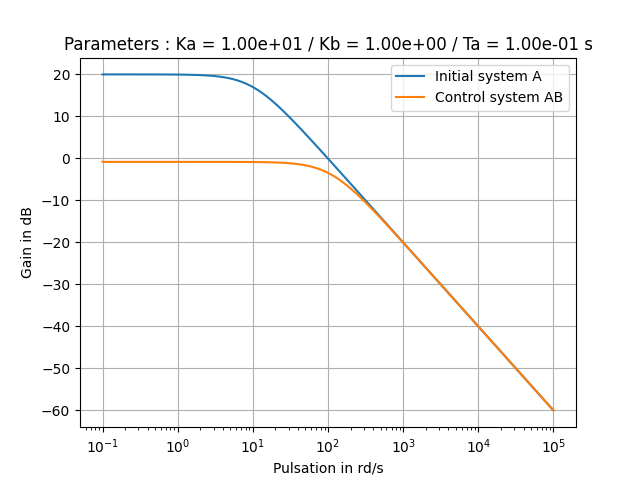
\includegraphics[width=0.5\textwidth]{images/A_1_B_0_bode_ex2.png}
	
	Exemple du système 2 : $K_A = 10$, $K_B = 1$ et $T_A = 100\operatorname{ms}$
\end{center}

\begin{center}
	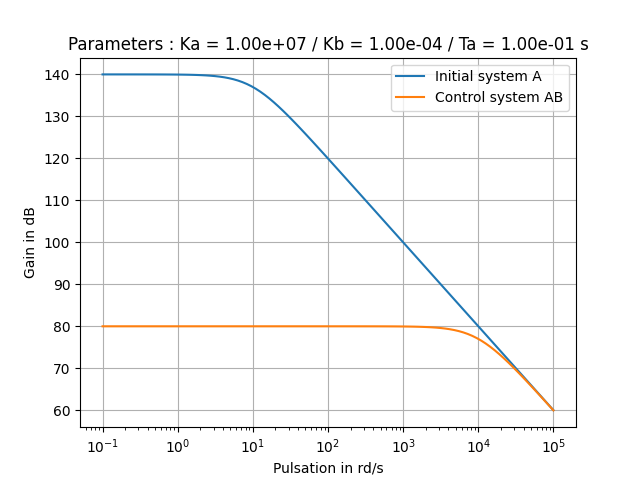
\includegraphics[width=0.5\textwidth]{images/A_1_B_0_bode_ALI.png}
	
	Exemple du système 3 : $K_A = 10^7$, $K_B = 10^{-4}$ et $T_A = 100\operatorname{ms}$
\end{center}

\newpage
\textbf{Et si A est d'ordre 2 ?}

De type : 

$$\boxed{H(j \omega) = \frac{K_A}{1 + 2 m j \frac{\omega}{\omega_0} + \frac{\omega^2}{\omega_0^2}}}$$

\begin{center}
	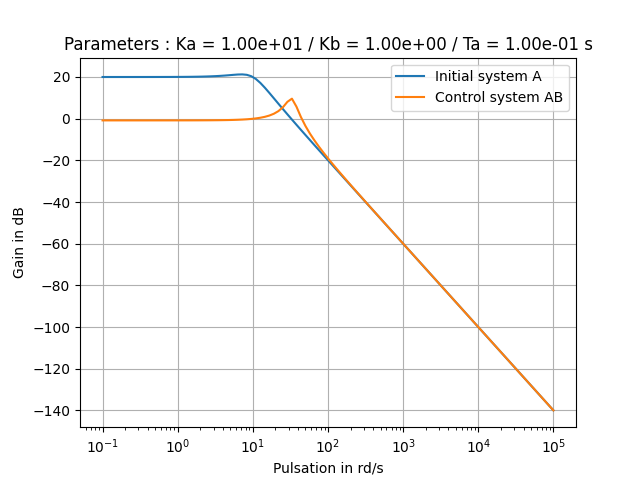
\includegraphics[width=0.5\textwidth]{images/A_2_B_0_bode_ex2.png}
	
	Exemple du système 2 : $K_A = 10$, $m = 0.5$, $K_B = 1$ et $T_A = 100\operatorname{ms}$
\end{center}


\begin{center}
	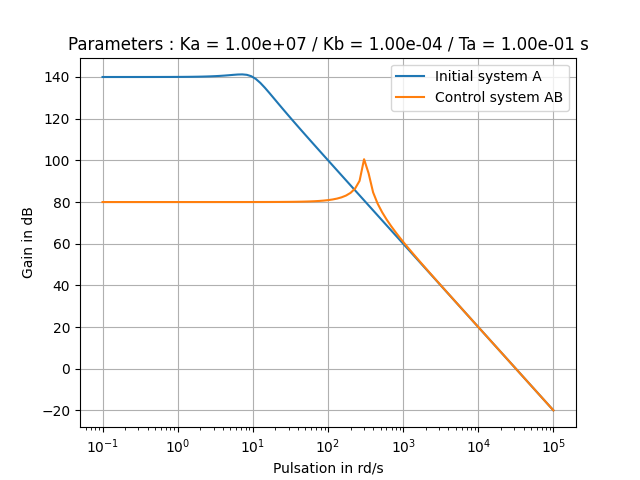
\includegraphics[width=0.5\textwidth]{images/A_2_B_0_bode_ALI.png}
	
	Exemple du système 3 (ALI) : $K_A = 10^7$, $m=0.5$, $K_B = 10^{-4}$ et $T_A = 100\operatorname{ms}$
\end{center}


\newpage
%%%%%%%%%%%%%%%%%%%%%%%%%%%%%%%%%%%%%%%%%%%%%%%%%%%%%%%
\subsection{Exercice 3 - Boucle ouverte et boucle fermée - Ordre 1}

Pour cet exercice, on considérera les fonctions de transfert suivantes : 

$A(j \omega) = K_A$ et $B(j \omega) = \frac{K_B}{1 + T_B j \omega}$

On donne l'expression suivante pour $H(j \omega) = G_S / G_E$ :

$$H(j \omega) = \frac{K_A}{1 + K_A K_B} \cdot \frac{1 + T_B j \omega}{1 + \frac{T_B}{1 + K_A K_B} j \omega}$$




\begin{enumerate}
	\item Tracez le gain de cette fonction de transfert dans les deux conditions suivantes :
	\begin{itemize}
		\item $K_A K_B > 1$
		\item $K_A K_B < 1$		
	\end{itemize}
	\item Donnez également l'expression du gain statique de ce système dans les deux conditions précédentes.
	\item Donnez également l'expression du rapport de la constante de temps du système bouclé sur celle du système A dans les deux conditions précédentes.
\end{enumerate}

%%%%%%%%%%%%%%%%%%%%%%
%%%%%%%%%%%%%%%%%%%%%%
\subsection*{Réponse}
%%%%%%%%%%%%%%%%%%%%%%
\medskip
\textbf{Question 1}

\begin{center}
	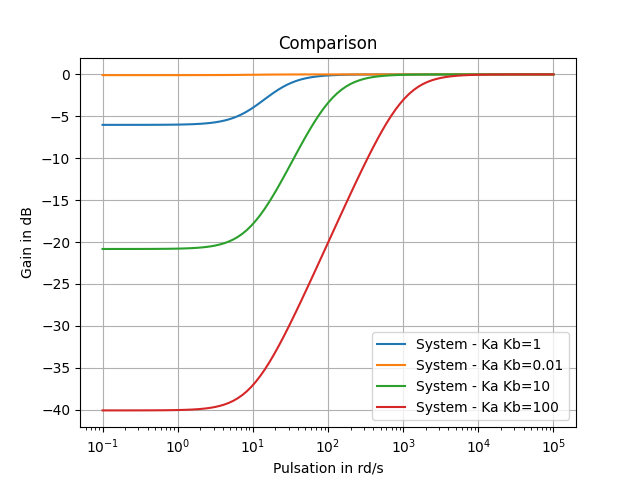
\includegraphics[width=0.5\textwidth]{images/A_0_B_1_bode_comp.png}
	
	Comparaison du diagramme de Bode en gain en fonction du produit des paramètres $K_A$ et $K_B$
\end{center}

\noindent\hrulefill

%%%%%%%%%%%%%%%%%%%%%%
\medskip
\textbf{Question 2}

On trouve : $$H_0 = \frac{K_A}{1 + K_A K_B}$$

Si $K_A K_B >> 1$ alors $H_0 \to 1/K_B$

Si $K_A K_B << 1$ alors $H_0 \to K_A$


\noindent\hrulefill

%%%%%%%%%%%%%%%%%%%%%%
\medskip
\textbf{Question 3}


On trouve : $$R = \frac{\frac{T_B}{1 + K_A K_B}}{T_B} = \frac{1}{1 + K_A K_B}$$

Si $K_A K_B >> 1$ alors $R \to \frac{1}{K_A K_B} \to 0$

Si $K_A K_B << 1$ alors $R \to 1$

%%%%%%%%%%%%%%%%%%%%%%
%%%%%%%%%%%%%%%%%%%%%%
\newpage

Pour les exercices 4 et 5, on considérera le schéma bloc suivant :


\begin{center}
{\Large
\begin{tikzpicture}
\sbEntree{E}
\sbComp{comp}{E}
\sbRelier[$G_E$]{E}{comp}
\sbStyleBloc{fill=schema_PID}
\sbBloc{reg}{$C(j \omega)$}{comp}
\sbRelier[$\varepsilon$]{comp}{reg}
\sbStyleBloc{fill=schema_action}
\sbBloc{sys}{$A(j \omega)$}{reg}
\sbStyleBlocDefaut
\sbRelier[$G_u$]{reg}{sys}
\sbSortie{S}{sys}
\sbRelier[$G_S$]{sys}{S}
\sbDecaleNoeudy[4]{S}{U}
\sbStyleBloc{fill=schema_feed}
\sbBlocr{cap}{$B(j \omega)$}{U}
\sbStyleBlocDefaut
\sbRelieryx{sys-S}{cap}
\sbRelierxy[$G_M$]{cap}{comp}
\end{tikzpicture}
}
\end{center}


%%%%%%%%%%%%%%%%%%%%%%%%%%%%%%%%%%%%%%%%%%%%%%%%%%%%%%%
\subsection{Exercice 4 - Correcteur P}

Pour cet exercice, on considérera les fonctions de transfert suivantes : 

$A(j \omega) = \frac{K_A}{1 + T_A j \omega}$, $B(j \omega) = K_B$ et $C(j \omega) = K_C$ 

\begin{enumerate}
	\item Donnez l'expression de $G_M$ en fonction de $G_E$, en \textbf{boucle ouverte}.
		
	\item Donnez l'expression de la \textbf{fonction de transfert} $H(j \omega) = G_S / G_E$, en \textbf{boucle fermée}.
	\item Mettez cette expression sous \textbf{forme canonique} et donnez les \textbf{principales caractéristiques} du système obtenu.
	\item Calculez ces valeurs caractéristiques pour les valeurs suivantes de $K_A$, $K_B$ et $T_A$ :
	\begin{itemize}
		\item $K_A = 1$, $K_B = 1$, $K_C = 10$ et $T_A = 100\operatorname{ms}$
		\item $K_A = 1$, $K_B = 10^{-2}$, $K_C = 10$ et $T_A = 100\operatorname{ms}$
	\end{itemize}
\end{enumerate}




%%%%%%%%%%%%%%%%%%%%%%
%%%%%%%%%%%%%%%%%%%%%%
\subsection*{Réponse}

%%%%%%%%%%%%%%%%%%%%%%
\medskip
\textbf{Question 1}

En boucle ouverte, $\varepsilon = G_E$ (le lien entre $G_M$ et le comparateur est ouvert).

On a alors : $\boxed{G_S = A(j \omega) C(j \omega) G_E}$

Et $\boxed{G_M = A(j \omega) B(j \omega) C(j \omega) G_E}$


\noindent\hrulefill

%%%%%%%%%%%%%%%%%%%%%%
\medskip
\textbf{Question 2}

En boucle fermée : 

\begin{itemize}
	\item $\varepsilon = G_E - G_M$
	\item $G_M = B(j \omega) G_S$
	\item $G_S = A(j \omega) C(j \omega) \varepsilon$
\end{itemize}

On obtient : $$\boxed{H(j \omega) = \frac{A(j \omega) C(j \omega)}{1 + A(j \omega) B(j \omega) C(j \omega)}}$$


En remplaçant $A(j \omega)$, $B(j \omega)$ et $C(j \omega)$ par leurs expressions, on trouve : $$\boxed{H(j \omega) = \frac{K_A K_C}{1 + K_A K_B K_C + T_A j \omega}} $$


\newpage
%%%%%%%%%%%%%%%%%%%%%%
\medskip
\textbf{Question 3}

La mise sous forme canonique (fonction de transfert de type passe-bas du premier ordre) donne l'expression suivante : $$\boxed{H(j \omega) = \frac{K_A K_C}{1 + K_A K_B K_C} \frac{1}{1 + \frac{T_A}{1 + K_A K_B K_C} j \omega}}$$

\medskip

On peut alors donner la constante de temps de ce système et le gain statique :

$$\boxed{T_H = \frac{T_A}{1 + K_A K_B K_C}}$$

$$\boxed{H_0 = \frac{K_A K_C}{1 + K_A K_B K_C}}$$


\noindent\hrulefill

%%%%%%%%%%%%%%%%%%%%%%
\medskip
\textbf{Question 4}

\underline{Pour $K_A = 1$, $K_B = 1$, $K_C = 10$ et $T_A = 100\operatorname{ms}$} :

$T_H = \frac{100\operatorname{ms}}{1 + 10} = 9\operatorname{ms}$

$H_0 = \frac{10}{11}$

\medskip

\underline{Pour $K_A = 1$, $K_B = 10^{-2}$, $K_C = 10$ et $T_A = 100\operatorname{ms}$} :

$T_H = \frac{100\operatorname{ms}}{1 + 10^{-1}} = \frac{10}{11} \times 100\operatorname{ms} \approx 90\operatorname{ms}$

$H_0 = \frac{100}{11}$

%%%%%%%%%%%%%%%%%%%%%%
\textbf{Diagramme de Bode}

\begin{center}
	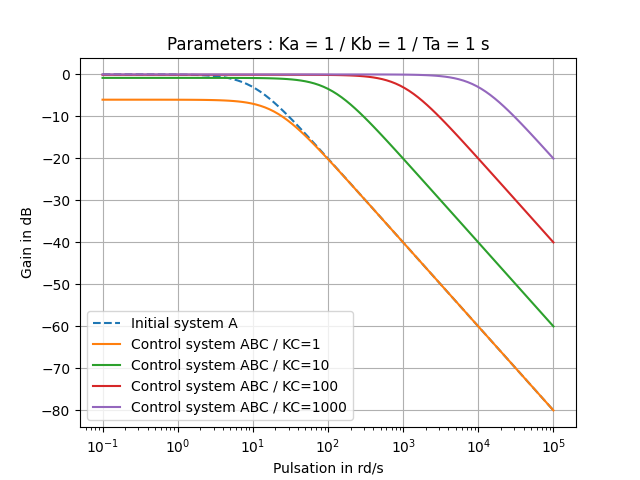
\includegraphics[width=0.5\textwidth]{images/A_1_B_0_C_0_bode_comp1.png}
	
	Comparaison du diagramme de Bode en gain en fonction de la valeur du gain du correcteur proportionnel ($K_C$)
\end{center}


%%%%%%%%%%%%%%%%%%%%%%
\bigskip
\bigskip
\textbf{Conclusion sur rebouclage et correcteur}

Le rebouclage (ou asservissement) a pour effet :

\begin{itemize}
	\item une vue sur la sortie
	\item une fonction de transfert du système global qui dépend du système à piloter et du système de mesure
\end{itemize}

Ce rebouclage impacte le \textbf{gain du montage} global et le \textbf{temps de réponse} global du montage.

L'ajout d'un \textbf{correcteur} (gain pour l'instant) permet de réduire l'erreur statique (pour un correcteur proportionnel $K_C \to \infty$) et de réduire le temps de réponse.


\newpage

%%%%%%%%%%%%%%%%%%%%%%%%%%%%%%%%%%%%%%%%%%%%%%%%%%%%%%%
\subsection{Exercice 5 - Correcteur PI}

Pour cet exercice, on considérera les fonctions de transfert suivantes : 

$A(j \omega) = \frac{K_A}{1 + T_A j \omega}$, $B(j \omega) = K_B$ et $C(j \omega) = K_C + \frac{1}{T_I j \omega}$ 

\bigskip

\begin{enumerate}
	\item Comparez les diagrammes de Bode en gain et les réponses indicielles suivants.
	\item Concluez sur le rôle des correcteurs proportionnel et intégral.
\end{enumerate}

\newpage
\begin{center}
	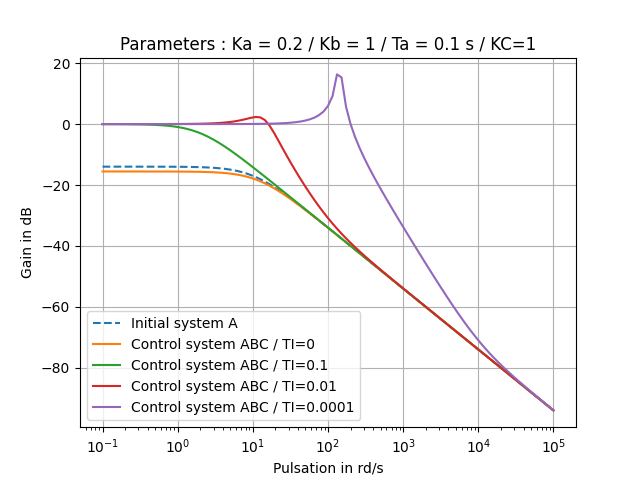
\includegraphics[width=0.8\textwidth]{images/A_0_B_0_CI_1_bode_comp1.png}
	
	Comparaison du diagramme de Bode en gain en fonction de la constante de temps de l'intégrateur - $K_C = 1$.
\end{center}

\begin{center}
	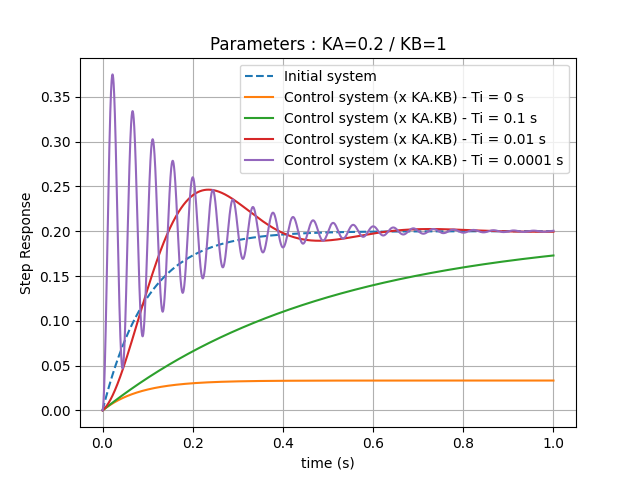
\includegraphics[width=0.8\textwidth]{images/A_0_B_0_CI_1_step_comp1.png}
	
	Comparaison de la réponses indicielle en fonction de la constante de temps de l'intégrateur - $K_C = 1$.
\end{center}


\newpage
\begin{center}
	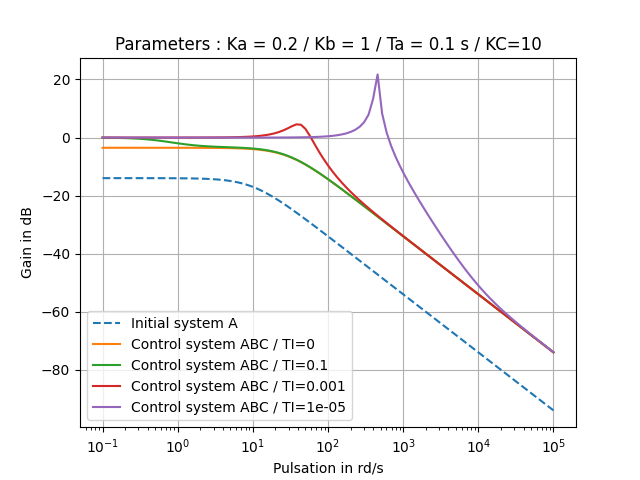
\includegraphics[width=0.8\textwidth]{images/A_0_B_0_CI_1_bode_comp2.png}
	
	Comparaison du diagramme de Bode en gain en fonction de la constante de temps de l'intégrateur - $K_C = 10$.
\end{center}

\begin{center}
	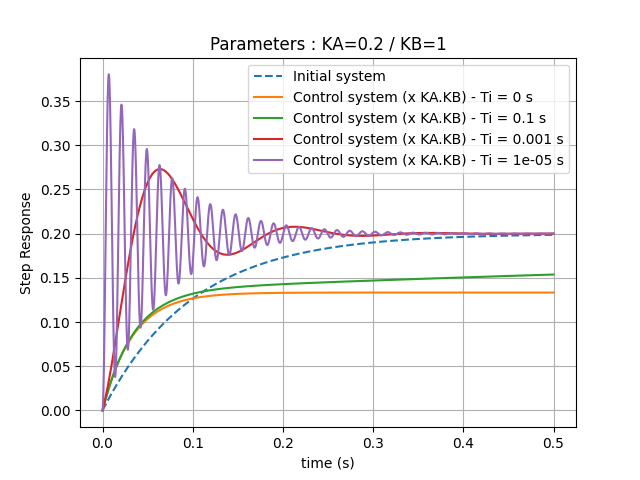
\includegraphics[width=0.8\textwidth]{images/A_0_B_0_CI_1_step_comp2.png}
	
	 Comparaison de la réponses indicielle en fonction de la constante de temps de l'intégrateur - $K_C = 10$.
\end{center}

%%%%%%%%%%%%%%%%%%%%%%%%%%%%%%%%%%%%%%%%%%%%%%%%%%%%%%%


\end{document}


